\documentclass[border=5pt]{standalone}
\usepackage{tikz}
\usepackage{amsmath}
\begin{document}
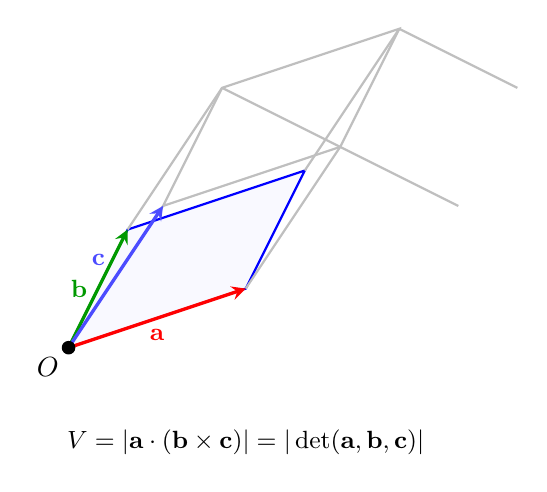
\begin{tikzpicture}[scale=1.5, >=stealth]
  % Parallelepiped from 3 vectors (determinant = volume)

  % Back face
  \draw[thick, gray!50] (0.8, 1.2) -- (2.3, 1.7) -- (2.8, 2.7) -- (1.3, 2.2) -- cycle;
  \draw[thick, gray!50] (2.3, 1.7) -- (3.3, 1.2);
  \draw[thick, gray!50] (2.8, 2.7) -- (3.8, 2.2);
  \draw[thick, gray!50] (1.3, 2.2) -- (2.3, 1.7);

  % Front face
  \fill[blue!8, opacity=0.3] (0,0) -- (1.5,0.5) -- (2,1.5) -- (0.5,1) -- cycle;
  \draw[thick, blue] (0,0) -- (1.5,0.5) -- (2,1.5) -- (0.5,1) -- cycle;

  % Connecting edges
  \draw[thick, gray!50] (0,0) -- (0.8,1.2);
  \draw[thick, gray!50] (1.5,0.5) -- (2.3,1.7);
  \draw[thick, gray!50] (2,1.5) -- (2.8,2.7);
  \draw[thick, gray!50] (0.5,1) -- (1.3,2.2);

  % Vectors from origin
  \draw[->, very thick, red] (0,0) -- (1.5,0.5) node[midway, below, font=\small] {$\mathbf{a}$};
  \draw[->, very thick, green!60!black] (0,0) -- (0.5,1) node[midway, left, font=\small] {$\mathbf{b}$};
  \draw[->, very thick, blue!70] (0,0) -- (0.8,1.2) node[midway, above left, font=\small] {$\mathbf{c}$};

  % Origin
  \filldraw[black] (0,0) circle (1.5pt) node[below left] {$O$};

  % Formula
  \node[font=\small] at (1.5, -0.8) {$V = |\mathbf{a}\cdot(\mathbf{b}\times\mathbf{c})| = |\det(\mathbf{a},\mathbf{b},\mathbf{c})|$};
\end{tikzpicture}
\end{document}
